\chapter{基于 TLA+ 的 OT函数验证} 
\section{TLA+ 简介}
\par TLA+是一种形式化的规范语言。它是一种设计系统和算法的工具,并且用来验证这些系统有没有关键错误。
\par 正确性,是一个系统最为重要的性质,同时,正确性是比较难以证明的,特别是并发系统的正确性,因为存在着数目众多的状态变化,而TLA+可以将系统的行为或者状态抽象为时态逻辑,即系统的行为或者状态会随着时间反生变化,然后通过一些数学分析的方法,来判断系统是否正确。
\par TLA+并不同于一般传统意义上的编程语言,更类似于一种数学语言,因为其语法大部分来自于实际的数理逻辑。
\par TLA+提供了工具集TLAToolbox/TLC,同时还可以使用TLA+的语法糖PLUSCAL来完成代码的编写,由于本文中并未涉及,在此不做展开。
\begin{figure}
\centering
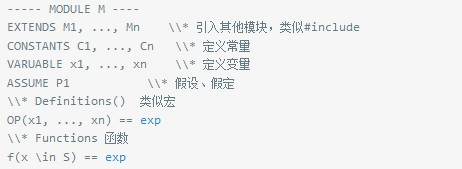
\includegraphics{figures/module.jpg}
\caption{TLA+编码模板}
\label{fig:graph}
\end{figure}

\section{使用 TLA+ 描述 OT 函数}
\subsection{调用模块的简单介绍}
\par 在本次实验中,我们引入了TLA+ 中的Sequences模块,将List表示为一个Sequecnce,并且使用了如下的API:\\
\begin{tabular}{ccc}
\hline
operator& operation& example \\
\hline  
 Head& First element &Head(<<1, 2>>) = 1\\
 Tail& Sequence aside from head &Tail(<<1, 2>>) = <<2>>\\
 Append& Add element to end of sequence &Append(<<1>>, 2) = <<1, 2>>\\ 
 Len& Length of sequence &Len(<<1, 2>>) = 2\\
\hline % 
\end{tabular}
 	 	
\subsection{OT函数设计}
\paragraph{第一、二类函数的表示}
\paragraph{第三、四类函数的表示}
\paragraph{命令执行的表示}

\section{正确性验证}
\par 在第二章中,我们提到过CP1和CP2两个协议,在这里我们只验证CP1性质的正确性。即同一个List经过OT(OP2,OP1),OP1或者OT(OP1,OP2),OP1这两种操作序列后,最终的结果是一致的。
\par 用TLA+来描述就是:
\par $apply(apply(list,op1),Xform(op2, op1)) = apply(apply(list,op2),Xform(op1, op2)) $
\par 只要对于任意的两个操作,这个等式都成立的话,那么CP1正确性即可得到验证。